\chapter{Guía de Inicio Rápido para Usuarios}
\label{AppendixD}

Este apéndice constituye una guía operativa dirigida al personal docente y administrativo de la FACET para el uso cotidiano de la plataforma de firma electrónica Documenso. Se describen los pasos necesarios para firmar documentos institucionales dentro del contexto organizacional correcto. Para funcionalidades avanzadas ---plantillas, enlaces directos reutilizables, configuración de equipos--- se recomienda consultar la documentación oficial del proyecto, disponible en \url{https://docs.documenso.com/docs/users}.

%----------------------------------------------------------------------------------------

\section{Acceso al Sistema}
\label{AppendixD:Acceso}

El acceso se realiza mediante autenticación Google OAuth con la cuenta institucional @herrera.unt.edu.ar. Al iniciar sesión por primera vez, el sistema posiciona al usuario en su organización \textbf{Personal}, que es un espacio individual no vinculado a la estructura institucional. Los documentos creados en este espacio no se asocian a la FACET.

%----------------------------------------------------------------------------------------

\section{Selección de Organización y Equipo}
\label{AppendixD:OrgTeam}

\textbf{Este es el paso más importante del flujo de trabajo.} Antes de cargar cualquier documento oficial, se debe verificar el contexto organizacional:

\begin{enumerate}[nosep]
    \item En el selector de organización (ubicado en la barra superior derecha), cambiar de \textbf{Personal} a \textbf{FACET} (Figura~\ref{fig:apD_selector_org}).
    \item Una vez dentro de la organización FACET, seleccionar el \textbf{Equipo} (Departamento) correspondiente al departamento del usuario (Figura~\ref{fig:apD_selector_team}).
\end{enumerate}

Todo documento subido fuera del contexto FACET/Equipo quedará desvinculado de la estructura institucional y no será visible para los demás miembros del departamento.

\textbf{Si la organización FACET no aparece en el selector,} cerrar la sesión actual, abrir el enlace de invitación a la organización FACET recibido por correo electrónico e iniciar sesión nuevamente con la cuenta institucional. Tras este paso, la organización FACET quedará disponible en el selector.

\begin{figure}[H]
    \centering
    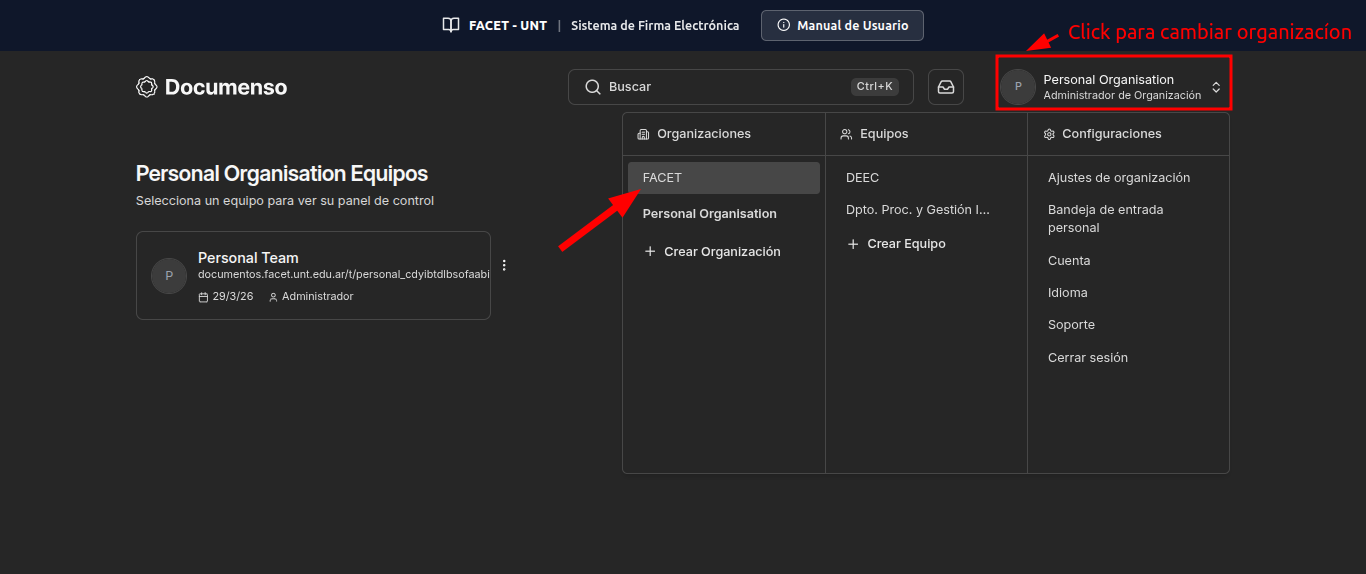
\includegraphics[width=0.8\textwidth]{figuras/apendiceD/selector-org-facet.png}
    \caption[Selector de organización]{Selector de organización desplegado. Se debe cambiar de \emph{Personal} a \emph{FACET} antes de operar con documentos institucionales.}
    \label{fig:apD_selector_org}
\end{figure}

\begin{figure}[H]
    \centering
    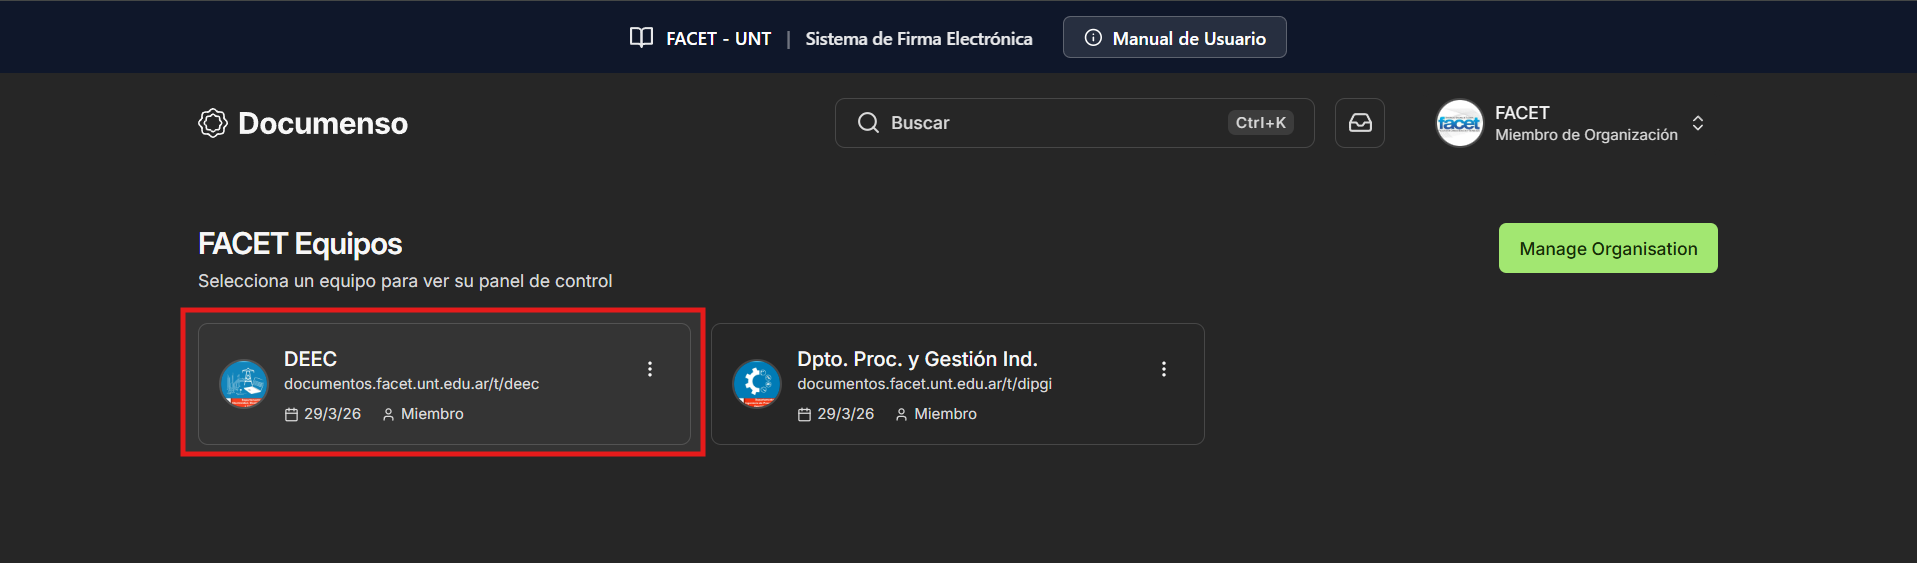
\includegraphics[width=0.8\textwidth]{figuras/apendiceD/selector-team.png}
    \caption[Selector de equipo dentro de FACET]{Listado de equipos dentro de la organización FACET. Cada equipo corresponde a un departamento o área de la facultad.}
    \label{fig:apD_selector_team}
\end{figure}

%----------------------------------------------------------------------------------------

\section{Carga y Preparación de un Documento}
\label{AppendixD:CargaDocumento}

\subsection{Carga del Archivo}
\label{AppendixD:CargaArchivo}

Desde el panel de documentos del equipo, utilizar el botón \textbf{Cargar Documento} para subir el archivo PDF a firmar (Figura~\ref{fig:apD_cargar_doc}). El sistema presenta dos opciones: se debe seleccionar \textbf{Cargar Documento} e ignorar la opción \emph{Documento (Legado)}. El tamaño máximo admitido es de 50\,MB y el formato aceptado es exclusivamente PDF.

\begin{figure}[H]
    \centering
    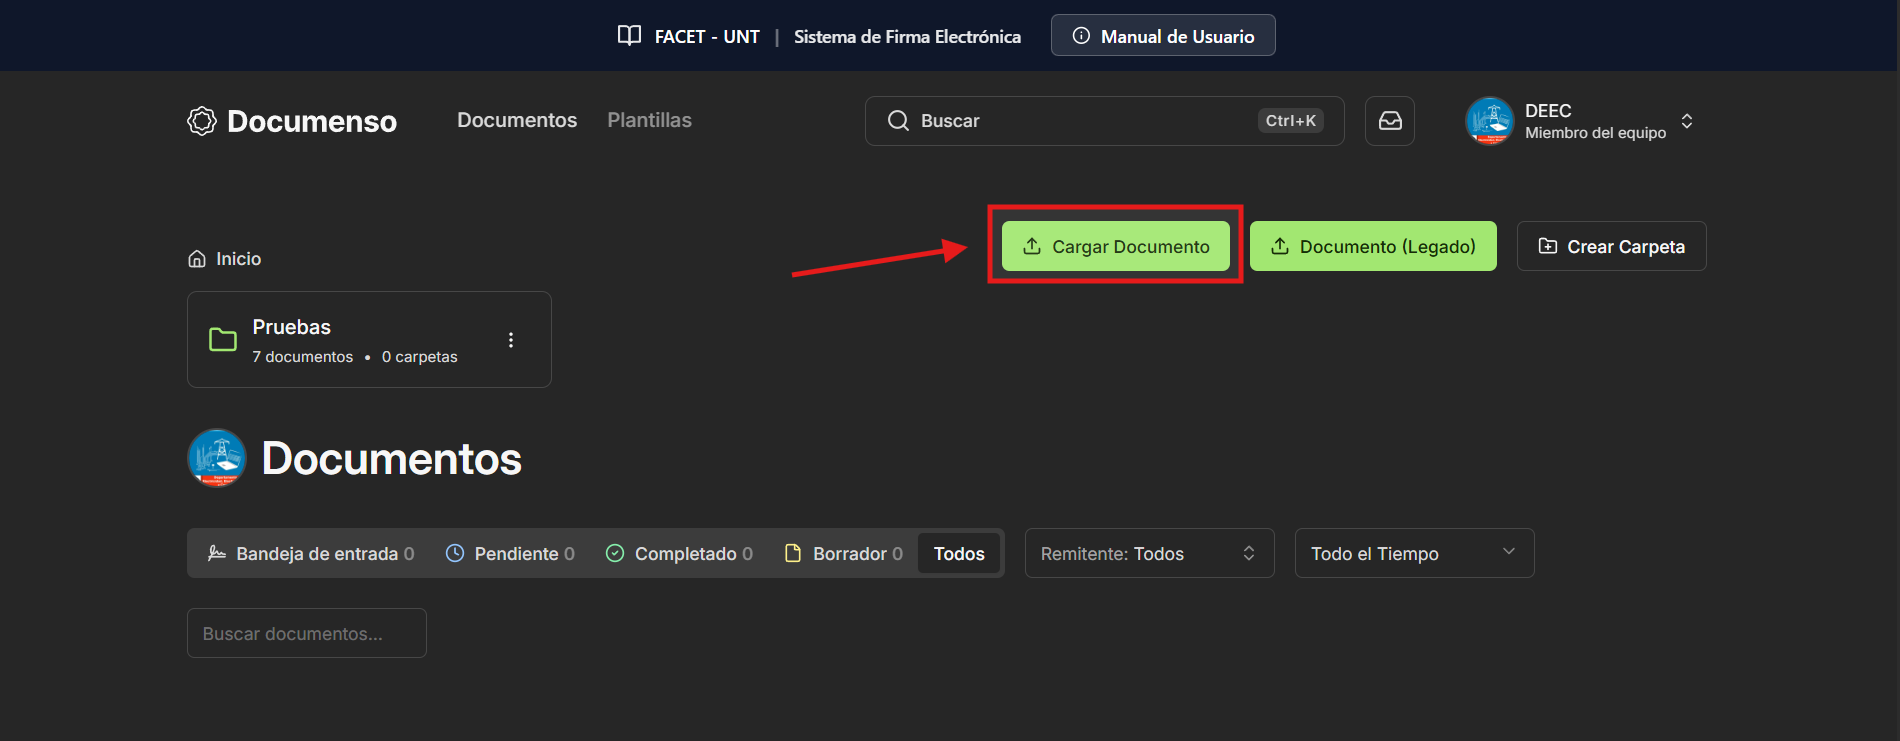
\includegraphics[width=0.8\textwidth]{figuras/apendiceD/boton-cargar-documento.png}
    \caption[Opciones de carga de documento]{Opciones de carga. Seleccionar siempre \emph{Cargar Documento}; la opción \emph{Documento (Legado)} no debe utilizarse.}
    \label{fig:apD_cargar_doc}
\end{figure}

Una vez cargado, el documento ingresa en estado \textbf{Borrador} y se accede al editor de preparación.

\subsection{Destinatarios y Roles}
\label{AppendixD:Destinatarios}

En el editor, se agregan los destinatarios indicando para cada uno su dirección de correo electrónico, nombre y rol. La Tabla~\ref{tab:apD_roles} resume los roles disponibles.

\begin{table}[H]
\centering
\caption{Roles de destinatario disponibles en Documenso.}
\label{tab:apD_roles}
\begin{tabular}{l l p{7.5cm}}
\hline
\textbf{Rol} & \textbf{¿Acción requerida?} & \textbf{Descripción} \\
\hline
Firmante   & Sí & Debe completar los campos de firma asignados. \\
Aprobador  & Sí & Debe aprobar el documento; la firma es opcional. \\
Visor      & Sí & Debe confirmar que ha revisado el documento. \\
CC         & No & Recibe una copia del documento una vez completado. \\
\hline
\end{tabular}
\end{table}

Opcionalmente, se puede habilitar el \textbf{orden de firma} para que los destinatarios actúen en secuencia (por ejemplo, un aprobador en posición~1 y los firmantes en posición~2).

\subsection{Colocación de Campos de Firma}
\label{AppendixD:Campos}

En la sección \emph{Agregar Campos} del editor, se selecciona el destinatario en el panel lateral y se arrastra al menos un campo de tipo \textbf{Firma} sobre la zona del PDF donde debe estamparse (Figura~\ref{fig:apD_editor_campos}). Los campos se identifican por color según el destinatario asignado. Adicionalmente, se pueden colocar campos de nombre, fecha, texto, iniciales u otros tipos según la necesidad del documento.

\begin{figure}[H]
    \centering
    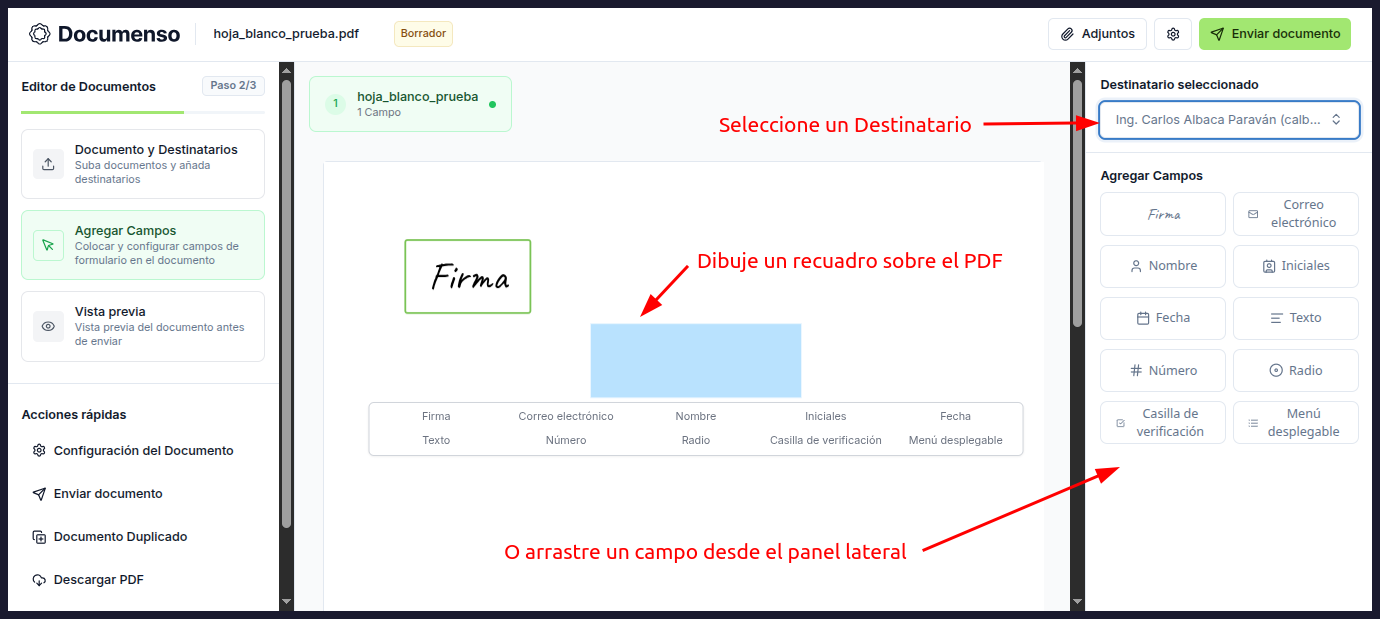
\includegraphics[width=0.85\textwidth]{figuras/apendiceD/editor-campos.png}
    \caption[Editor de campos de firma]{Editor de documento con un campo de firma colocado sobre el PDF. El panel lateral derecho muestra los tipos de campo disponibles.}
    \label{fig:apD_editor_campos}
\end{figure}

El documento no podrá enviarse hasta que cada firmante tenga asignado al menos un campo de firma.

%----------------------------------------------------------------------------------------

\section{Envío del Documento}
\label{AppendixD:Envio}

Una vez preparado el documento, se procede al envío. La plataforma ofrece dos modalidades de distribución:

\begin{enumerate}[nosep]
    \item \textbf{Correo electrónico:} cada destinatario recibe una notificación por correo con un enlace único de firma. Se puede personalizar el asunto y el cuerpo del mensaje.
    \item \textbf{Link Directo:} se genera un enlace de firma sin enviar correo. Esta modalidad es útil para distribuir el documento por WhatsApp, mensajería interna u otros canales.
\end{enumerate}

La Figura~\ref{fig:apD_envio} muestra ambas opciones en la pantalla de envío.

\begin{figure}[H]
    \centering
    \begin{subfigure}[b]{0.45\textwidth}
        \centering
        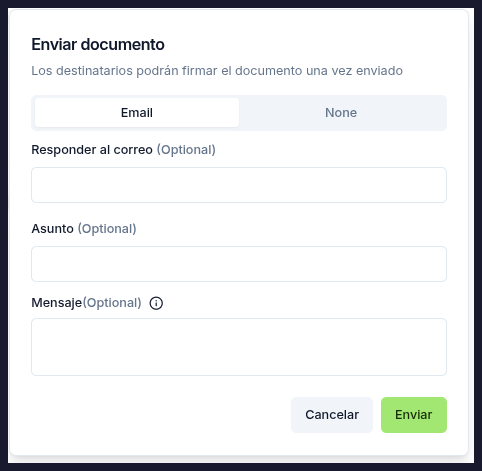
\includegraphics[width=\textwidth]{figuras/apendiceD/envio-modalidades-mail.png}
        \caption{Distribución por correo electrónico.}
        \label{fig:apD_envio_mail}
    \end{subfigure}
    \hfill
    \begin{subfigure}[b]{0.45\textwidth}
        \centering
        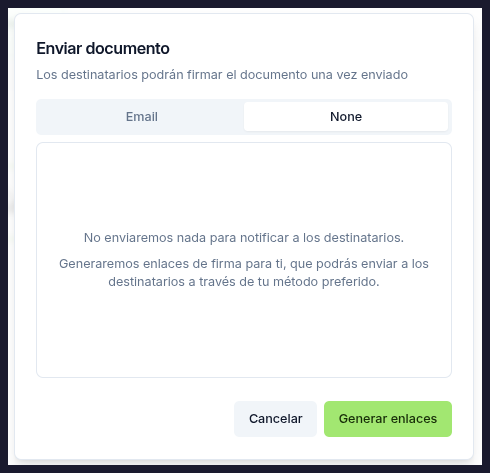
\includegraphics[width=\textwidth]{figuras/apendiceD/envio-modalidades-link.png}
        \caption{Generación de link directo de firma.}
        \label{fig:apD_envio_link}
    \end{subfigure}
    \caption[Modalidades de envío]{Pantalla de envío del documento. (a)~Distribución por correo electrónico. (b)~Generación de link directo de firma.}
    \label{fig:apD_envio}
\end{figure}

Tras el envío, el documento pasa del estado \emph{Borrador} a \textbf{Pendiente}.

%----------------------------------------------------------------------------------------

\section{Seguimiento y Finalización}
\label{AppendixD:Seguimiento}

El progreso de cada documento se puede consultar desde el panel de documentos del equipo. La Tabla~\ref{tab:apD_estados} describe los estados posibles.

\begin{table}[H]
\centering
\caption{Estados del ciclo de vida de un documento.}
\label{tab:apD_estados}
\begin{tabular}{l p{10cm}}
\hline
\textbf{Estado} & \textbf{Descripción} \\
\hline
Borrador    & El documento está en preparación; aún no ha sido enviado. \\
Pendiente   & El documento fue enviado y aguarda la acción de los destinatarios. \\
Completado  & Todos los destinatarios completaron sus acciones. El documento queda sellado con un certificado digital. \\
Rechazado   & Un destinatario rechazó el documento (si la opción de rechazo fue habilitada). El documento no puede modificarse ni reactivarse; es necesario crear uno nuevo. \\
\hline
\end{tabular}
\end{table}

Al completarse, todas las partes reciben una copia del PDF firmado y sellado digitalmente.

Si un destinatario no ha actuado sobre el documento, se le puede reenviar un recordatorio desde el menú de acciones (tres puntos) del documento en estado \emph{Pendiente}.

Para cancelar un envío erróneo, se puede eliminar el documento desde el mismo menú de acciones. Esta operación es irreversible: se anulan todas las firmas pendientes y los destinatarios reciben una notificación de cancelación.

%----------------------------------------------------------------------------------------

\section{Experiencia del Destinatario}
\label{AppendixD:Destinatario}

El destinatario accede al documento a través del enlace recibido por correo o por link directo. Al abrirlo, visualiza el PDF con sus campos asignados resaltados. Para los campos de firma, puede optar por dibujar la firma manualmente, escribir su nombre y seleccionar un estilo tipográfico, o cargar una imagen de su firma. Una vez completados todos los campos obligatorios, confirma la acción.
%----------------------------------------------------------------------------------------

\section{Referencia Rápida}
\label{AppendixD:Referencia}

A modo de síntesis, el flujo completo para documentos institucionales es:

\begin{enumerate}[nosep]
    \item Iniciar sesión con la cuenta \texttt{@herrera.unt.edu.ar}.
    \item Cambiar a la organización \textbf{FACET} y seleccionar el equipo del departamento.
    \item Cargar el PDF mediante \textbf{Cargar Documento}.
    \item Agregar destinatarios con sus roles y colocar los campos de firma.
    \item Enviar por correo electrónico o generar un link directo.
    \item Consultar el estado desde el panel de documentos.
\end{enumerate}

Para funcionalidades adicionales como la creación de plantillas reutilizables, la configuración de enlaces directos públicos o la gestión de equipos, consultar la documentación oficial de Documenso disponible en \url{https://docs.documenso.com/docs/users}.
